\usetikzlibrary{patterns}

\usetikzlibrary{arrows}
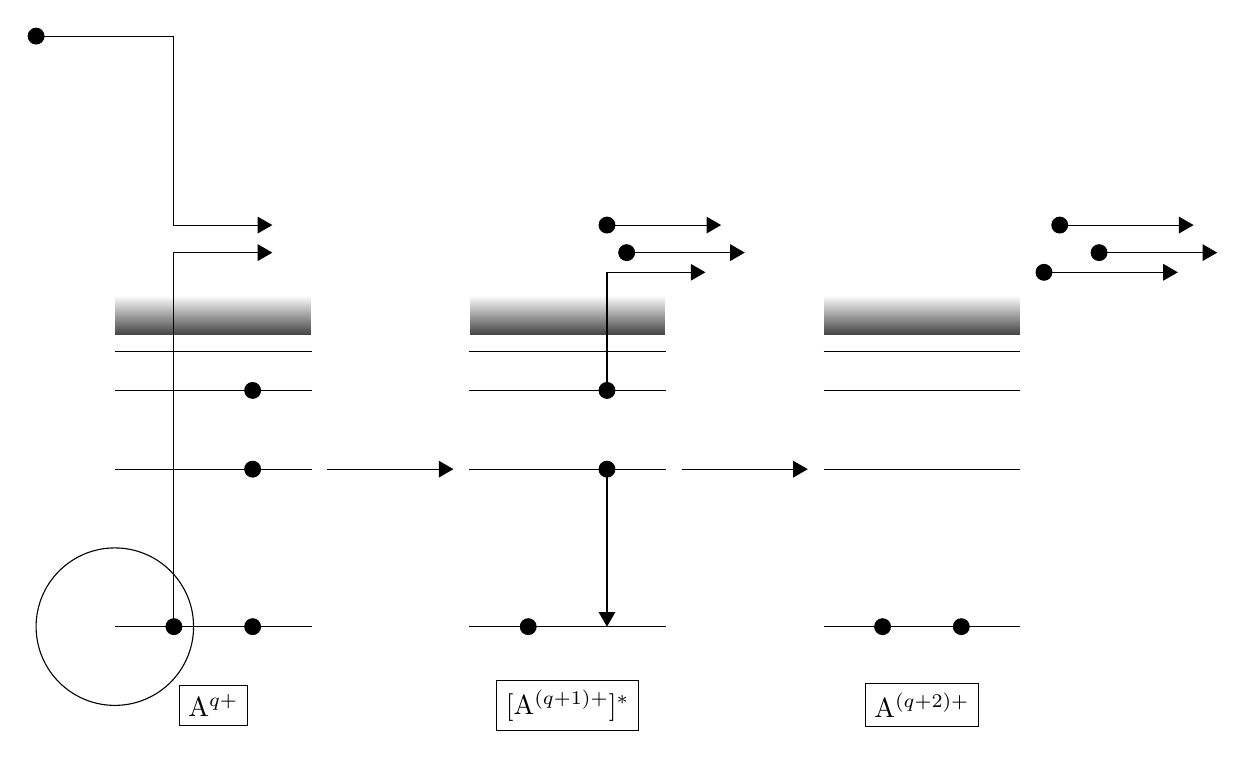
\begin{tikzpicture}
% Anker
\draw  (0,0) ellipse (1 and 1);
%

% Nr 1 Standard Darstellung ohne Elektronen
\draw (0,0) -- (2.5,0);
\draw (0,2) -- (2.5,2);
\draw (0,3) -- (2.5,3);
\draw (0,3.5) -- (2.5,3.5);
\shadedraw [draw=white,top color=lightgray!5,bottom color=darkgray] (0,3.7) rectangle (2.5,4.2);


% Nr 2 Standard Darstellung ohne Elektronen
\draw (4.5,0) -- (7,0);
\draw (4.5,2) -- (7,2);
\draw (4.5,3) -- (7,3);
\draw (4.5,3.5) -- (7,3.5);
\shadedraw [draw=white,top color=lightgray!5,bottom color=darkgray] (4.5,3.7) rectangle (7.0,4.2);


% Nr 3 Standard Darstellung ohne Elektronen
\draw (9,0) -- (11.5,0);
\draw (9,2) -- (11.5,2);
\draw (9,3) -- (11.5,3);
\draw (9,3.5) -- (11.5,3.5);
\shadedraw [draw=white,top color=lightgray!5,bottom color=darkgray] (9.0,3.7) rectangle (11.5,4.2);


% Pfeile
\draw[-triangle 60] (2.7,2) -- (4.3,2); % 1 nach 2
\draw[-triangle 60] (7.2,2) -- (8.8,2); % 2 nach 3


% Elektronen (von unten nach oben)
% Nr 1 Standard
\filldraw  (0.75,0) ellipse (0.1 and 0.1);
\filldraw  (1.75,0) ellipse (0.1 and 0.1);
\filldraw  (1.75,2.0) ellipse (0.1 and 0.1);
\filldraw  (1.75,3.0) ellipse (0.1 and 0.1);
\filldraw  (-1.0,7.5) ellipse (0.1 and 0.1); % Kontinuum Elektron


% Elektronen (von unten nach oben)
% Nr 2 Standard
\filldraw  (5.25,0) ellipse (0.1 and 0.1);
\filldraw  (6.25,2) ellipse (0.1 and 0.1);
\filldraw  (6.25,3) ellipse (0.1 and 0.1);
\filldraw  (6.5,4.75) ellipse (0.1 and 0.1); % erstes abgelöstes Elektronen, frei unten
\filldraw  (6.25,5.1) ellipse (0.1 and 0.1); % freies Elektron oben

% Elektronen (von unten nach oben)
% Nr 3 Standard
\filldraw  (9.75,0) ellipse (0.1 and 0.1);
\filldraw  (10.75,0) ellipse (0.1 and 0.1);
\filldraw  (11.8,4.5) ellipse (0.1 and 0.1); % % zweites abgelöstes Elektronen, frei unten
\filldraw  (12.5,4.75) ellipse (0.1 and 0.1); % erstes abgelöstes Elektronen, frei unten
\filldraw  (12,5.1) ellipse (0.1 and 0.1); % freies Elektron oben


% Elektronenweg
% Nr 1 Standard
\draw [-triangle 60](-1.0,7.5) -- (0.75,7.5) -- (0.75,5.1) -- (2.0,5.1); % Kontinuum Elektron
\draw [-triangle 60](0.75,0) -- (0.75,4.75) -- (2.0,4.75); % abgelöstes Elektron


% Elektronenweg
% Nr 2 Standard
\draw [-triangle 60](6.25,2) -- (6.25,0);
\draw [-triangle 60](6.25,3.0) -- (6.25,4.5) -- (7.5,4.5); % zweites abgelöstes Elektron
\draw [-triangle 60](6.5,4.75) -- (8,4.75); % erstes abgelöstes Elektron
\draw [-triangle 60](6.25,5.1) -- (7.7,5.1); % freie Elektronen

% Elektronenweg
% Nr 3 Standard
\draw [-triangle 60](11.8,4.5) -- (13.5,4.5) ; % zweites abgelöstes Elektron
\draw [-triangle 60](12.5,4.75) -- (14,4.75); % erstes abgelöstes Elektron
\draw [-triangle 60](12,5.1) -- (13.7, 5.1); % freie Elektronen





% Beschriftung
\node[draw] at (1.25,-1) {A$^{q+}$}; % 1
\node[draw] at (5.75,-1) {[A$^{(q+1)+}$]$^*$}; % 2
\node[draw] at (10.25,-1) {A$^{(q+2)+}$}; % 3


\end{tikzpicture}